\pdfinfo{%
  /Title    ()
  /Author   ()
  /Creator  ()
  /Producer ()
  /Subject  ()
  /Keywords ()
}

\section{Einleitung}
Der Nutzen der Administrator-Verwaltung besteht darin, dass bestimmte Nutzer mit exklusiven Rechten, die Möglichkeit haben, Aktionen, welche dazu dienen, den vernünftigen und guten Betrieb sicherzustellen, auszuführen.
Dazu dienen:
\begin{itemize}
 \item Gästebucheinträge freischalten, um Werbung bzw. unerlaubten Inhalt zu verhindern
 \item neuregistrierte Nutzer freischalten, um zu verhindern, dass sich Nutzer mehrmals anmelden bzw. die eingegebenen Daten überprüfgen zu können
 \item Nutzer löschen, um Nutzer, die sich falsch verhalten haben zu löschen
 \item Newseinträge löschen
\end{itemize}
Man erreicht die Administrator-Seite durch 2 Schritte
\begin{enumerate}
 \item einloggen mit einem Administrator-account z.B. Benutzername:``batman'', Passwort:``[input Passwort]''
 \item auswählen des Menüpunkts ``Admin-Verwaltung''
\end{enumerate}
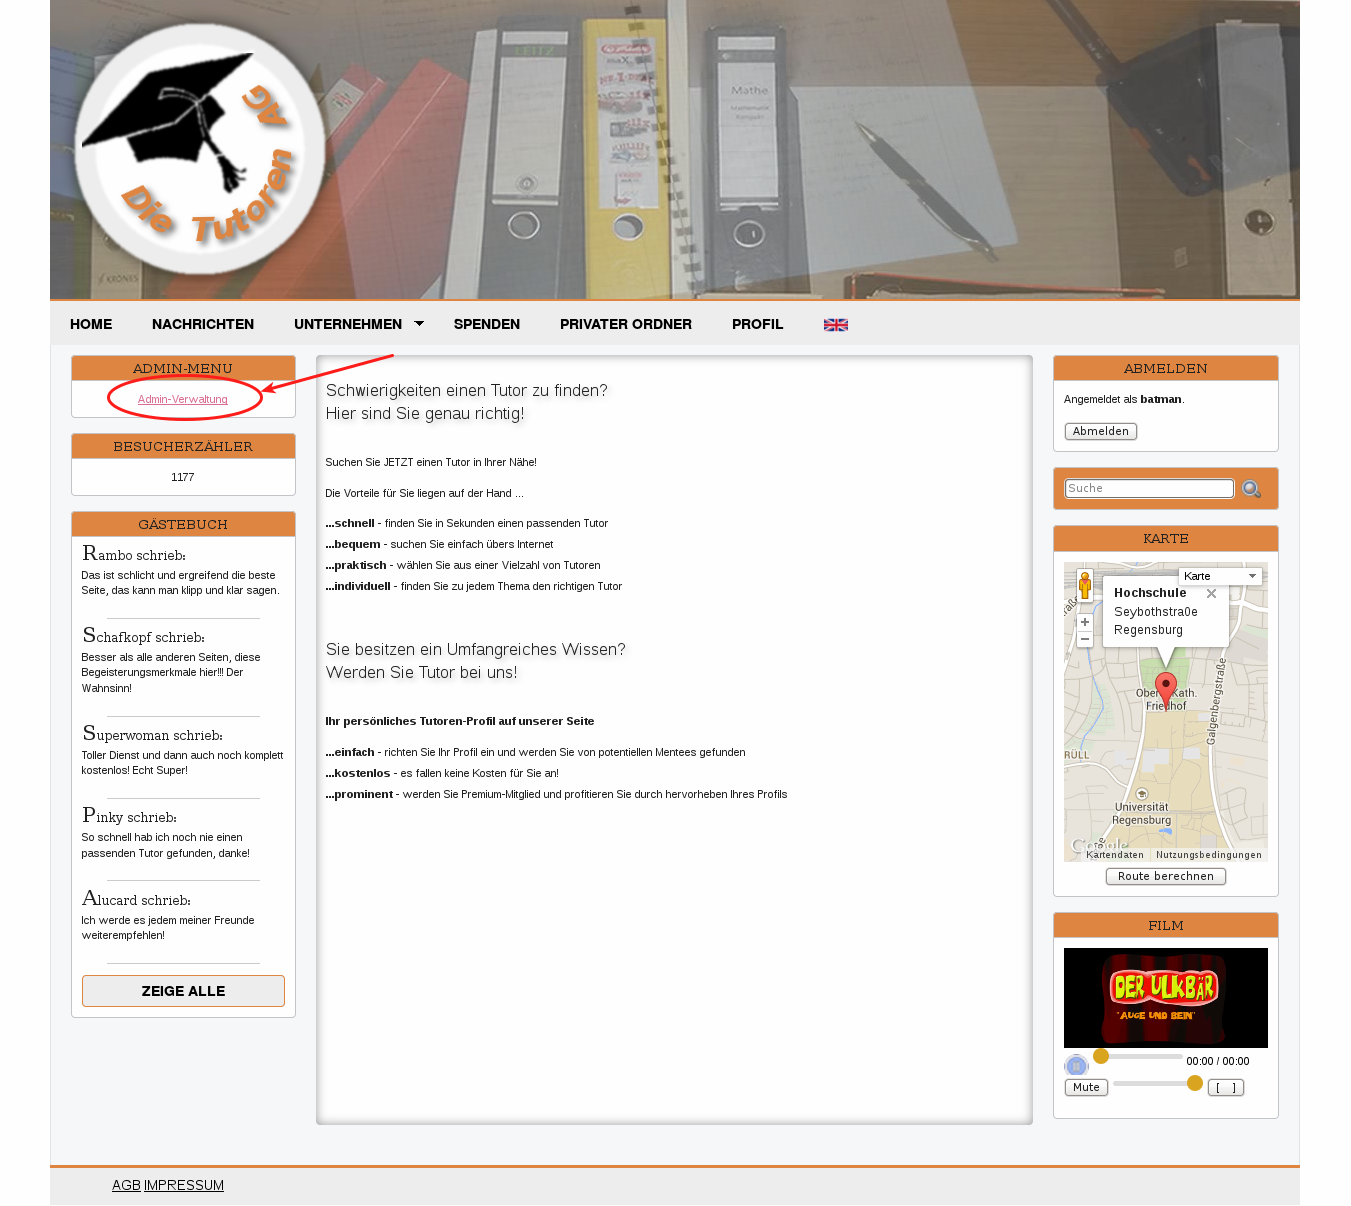
\includegraphics[width=1\textwidth]{../Screenshots/de/admin/Startseite_logged_in_admin}
\subsection{Landing-Page}
Dannach landet man auf der Landing-Page der Adminverwaltung, in der man die verschiedenen Menüpunkte durch klicken auswählen kann. Diese Punkte sind über alle Bereiche des Admin-Interface durch eine Schnellauswahl
erreichbar.\\
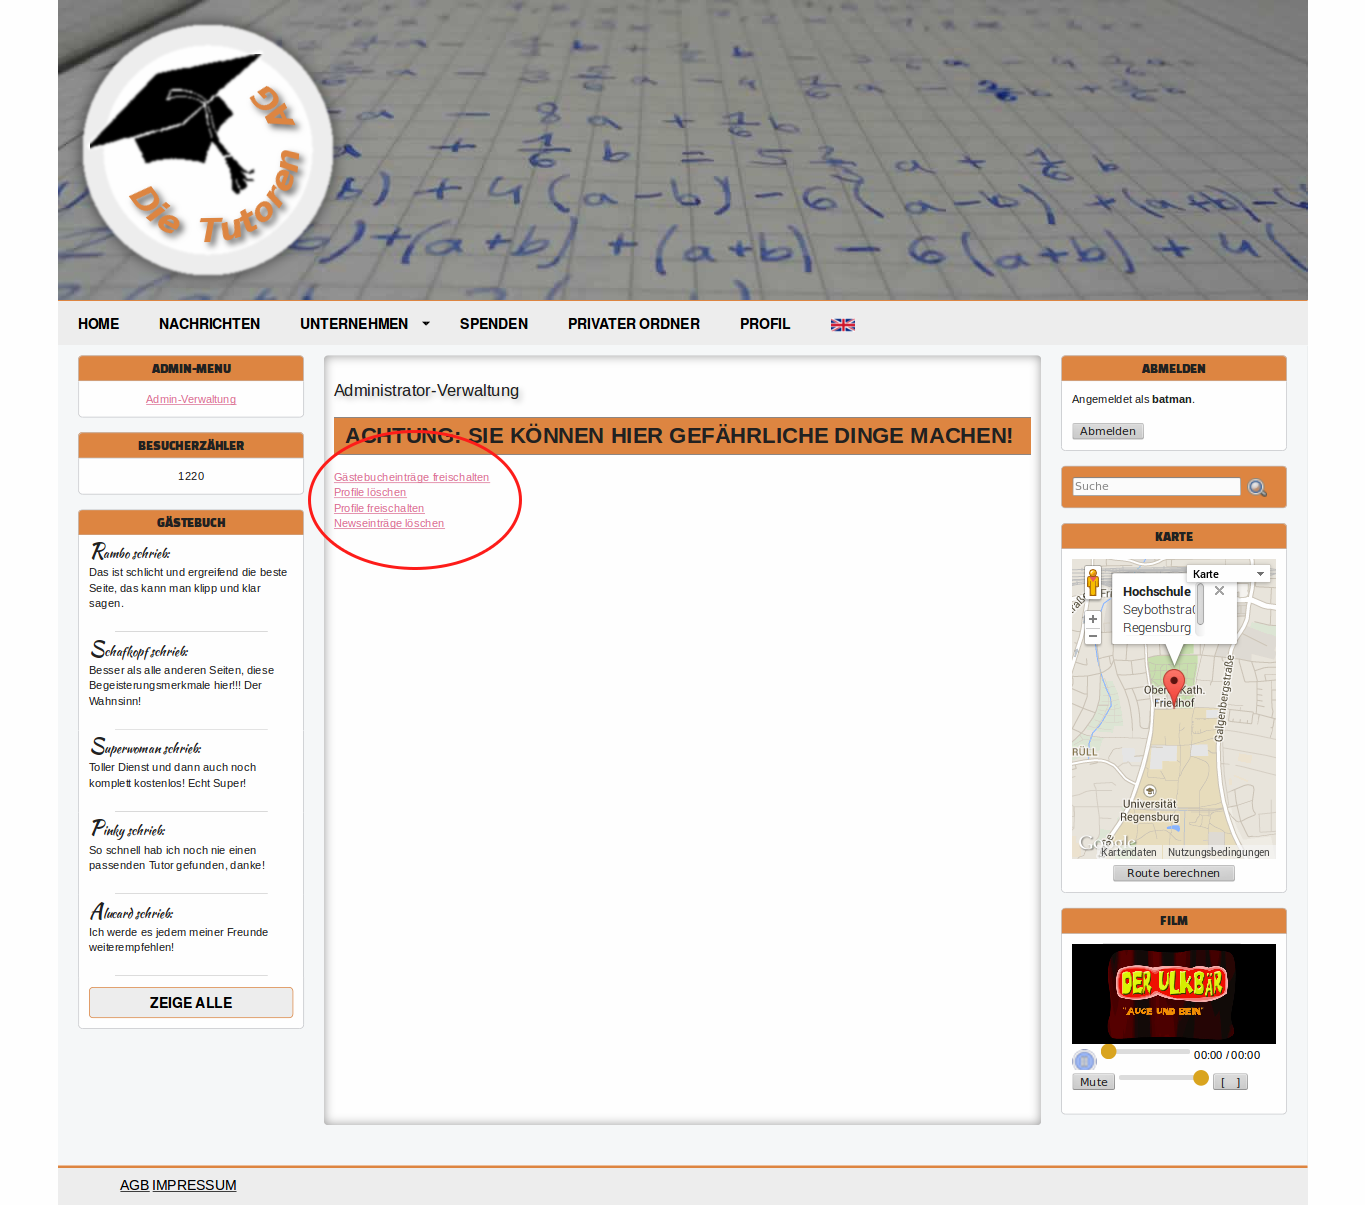
\includegraphics[width=1\textwidth]{../Screenshots/de/admin/admin_landing}

